% This template is indended for writting the the project report in ``Machine Learning``
%
% It is based on the MikTex ``article`` template, modified with content from the DIT ``Studienarbeit`` template, originally created by Prof. Dr. Andreas Fischer.
%
% Markus Mayer, 2022-03-23

\documentclass[11pt]{article} % use larger type; default would be 10pt
\usepackage[utf8]{inputenc} % set input encoding (not needed with XeLaTeX)

%%% Examples of Article customizations
% These packages are optional, depending whether you want the features they provide.
% See the LaTeX Companion or other references for full information.

%%% PAGE DIMENSIONS
\usepackage{geometry} % to change the page dimensions
\geometry{a4paper} % or letterpaper (US) or a5paper or....
% \geometry{margin=2in} % for example, change the margins to 2 inches all round
% \geometry{landscape} % set up the page for landscape
%   read geometry.pdf for detailed page layout information

\usepackage{graphicx} % support the \includegraphics command and options
\DeclareGraphicsExtensions{.pdf,.png,.jpg}

% \usepackage[parfill]{parskip} % Activate to begin paragraphs with an empty line rather than an indent

%%% PACKAGES
\usepackage{algorithmic} % For pseudo code
\usepackage{amsmath}
\usepackage{booktabs} % for much better looking tables
\usepackage{array} % for better arrays (eg matrices) in maths
\usepackage{paralist} % very flexible & customisable lists (eg. enumerate/itemize, etc.)
\usepackage{verbatim} % adds environment for commenting out blocks of text & for better verbatim
\usepackage{subfig} % make it possible to include more than one captioned figure/table in a single float
\usepackage{url}
\usepackage{hyperref}
\usepackage{float}
% These packages are all incorporated in the memoir class to one degree or another...

%%% HEADERS & FOOTERS
\usepackage{fancyhdr} % This should be set AFTER setting up the page geometry
\pagestyle{fancy} % options: empty , plain , fancy
\renewcommand{\headrulewidth}{0pt} % customise the layout...
\lhead{}\chead{}\rhead{}
\lfoot{}\cfoot{\thepage}\rfoot{}

%%% SECTION TITLE APPEARANCE
\usepackage{sectsty}
\allsectionsfont{\sffamily\mdseries\upshape} % (See the fntguide.pdf for font help)
% (This matches ConTeXt defaults)

%%% ToC (table of contents) APPEARANCE
\usepackage[nottoc,notlof,notlot]{tocbibind} % Put the bibliography in the ToC
\usepackage[titles,subfigure]{tocloft} % Alter the style of the Table of Contents
\renewcommand{\cftsecfont}{\rmfamily\mdseries\upshape}
\renewcommand{\cftsecpagefont}{\rmfamily\mdseries\upshape} % No bold!

%%% END Article customizations

%%% The "real" document content comes below...
\title{Project report on\\
popularity prediction of songs in Spotify and Youtube \\
}
\author{Omar Chafik, Santiago Lema}
\date{\today}

\begin{document}
\maketitle

\section{Introduction}
Throughout history, music has held a profound place in human society, transcending cultural boundaries and serving as a fundamental means of expression and engagement. From ancient tribal rituals to modern-day streaming platforms, music has always captivated our hearts and souls. It has the unique ability to evoke emotions, connect people, and create shared experiences. 

In today's digital age, the music industry has witnessed (and continues to witness) a deep transformation, where engagement and popularity on digital platforms play a crucial role in an artist's success. With millions of songs available on these platforms, understanding the factors that drive popularity and listeners' willingness to engage with a song is of great interest to artists, record labels, and other stakeholders in the music industry.

This project aims to delve into the realm of music popularity prediction, focusing on songs available on Spotify and YouTube, analyzing the relation between music features and users preferences. The goal will be pursued by developing  a classification model capable of predicting the popularity segment of a song, based on selected features. This entails constructing a comprehensive dataset containing various features and attributes of songs from the mentioned platforms. Leveraging such machine learning techniques, we will explore and compare multiple classification models to identify the most effective approach. Furthermore, we will fine-tune the selected models to extract the best possible results.

This is an exciting opportunity to merge music, data science and industry insights to gain a better understanding of the factors which give life to this ancient form of art. 

\section{Data}

The ground set of data for this project was obtained from a pre-built dataset available in Kaggle called \href{https://www.kaggle.com/datasets/salvatorerastelli/spotify-and-youtube}{\textit{Spotify and Youtube}}. The dataset contains 20.7128 songs with the following features:

\begin{table}[H]
	\centering
	\begin{tabular}{lcc}
		\toprule
		\textbf{Attribute} & \textbf{Unique values} & \textbf{Description} \\
		\midrule
		Artist & 2079 & Name of the artist \\
		Url\_spotify & 2079 & Spotify URL for the song \\
		Track & 17841 & Name of the track \\
		Album & 11937 & Name of the album \\
		Album\_type & 3 & Type of the album \\
		Uri & 18862 & URI of the song \\
		Danceability & 898 & Measure of the song's danceability \\
		Energy & 1268 & Measure of the song's energy \\
		Key & 12 & Key of the song \\
		Loudness & 9417 & Loudness level of the song \\
		Speechiness & 1303 & Measure of the song's speechiness \\
		Acousticness & 3138 & Measure of the song's acousticness \\
		Instrumentalness & 4012 & Measure of the song's instrumentalness \\
		Liveness & 1536 & Measure of the song's liveness \\
		Valence & 1293 & Measure of the song's valence \\
		Tempo & 15024 & Tempo of the song \\
		Duration\_ms & 14690 & Duration of the song in milliseconds \\
		Url\_youtube & 18154 & YouTube URL for the song \\
		Title & 18146 & Title of the YouTube video \\
		Channel & 6714 & YouTube channel of the uploader \\
		Views & 19245 & Number of views on YouTube \\
		Likes & 17939 & Number of likes on YouTube \\
		Comments & 10485 & Number of comments on YouTube \\
		Description & 17395 & Description of the YouTube video \\
		Licensed & 2 & Indicates if the song is licensed \\
		official\_video & 2 & Indicates if it's an official video \\
		Stream & 18461 & Indicates if the song is available for streaming \\
		\bottomrule
	\end{tabular}
	\caption{Attributes of the dataset}
	\label{tab:attributes}
\end{table}

\section{Method}

Lorem ipsum dolor sit amet, consetetur sadipscing elitr, sed diam nonumy eirmod tempor invidunt ut labore et dolore magna aliquyam erat, sed diam voluptua. At vero eos et accusam et justo duo dolores et ea rebum. Stet clita kasd gubergren, no sea takimata sanctus est Lorem ipsum dolor sit amet. Lorem ipsum dolor sit amet, consetetur sadipscing elitr, sed diam nonumy eirmod tempor invidunt ut labore et dolore magna aliquyam erat, sed diam voluptua. At vero eos et accusam et justo duo dolores et ea rebum. Stet clita kasd gubergren, no sea takimata sanctus est Lorem ipsum dolor sit amet. Lorem ipsum dolor sit amet, consetetur sadipscing elitr, sed diam nonumy eirmod tempor invidunt ut labore et dolore magna aliquyam erat, sed diam voluptua. At vero eos et accusam et justo duo dolores et ea rebum. Stet clita kasd gubergren, no sea takimata sanctus est Lorem ipsum dolor sit amet.   

Duis autem vel eum iriure dolor in hendrerit in vulputate velit esse molestie consequat, vel illum dolore eu feugiat nulla facilisis at vero eros et accumsan et iusto odio dignissim qui blandit praesent luptatum zzril delenit augue duis dolore te feugait nulla facilisi. Lorem ipsum dolor sit amet, consectetuer adipiscing elit, sed diam nonummy nibh euismod tincidunt ut laoreet dolore magna aliquam erat volutpat.   

Ut wisi enim ad minim veniam, quis nostrud exerci tation ullamcorper suscipit lobortis nisl ut aliquip ex ea commodo consequat. Duis autem vel eum iriure dolor in hendrerit in vulputate velit esse molestie consequat, vel illum dolore eu feugiat nulla facilisis at vero eros et accumsan et iusto odio dignissim qui blandit praesent luptatum zzril delenit augue duis dolore te feugait nulla facilisi.   

\section{Results and discussion}

Nam liber tempor cum soluta nobis eleifend option congue nihil imperdiet doming id quod mazim placerat facer possim assum. Lorem ipsum dolor sit amet, consectetuer adipiscing elit, sed diam nonummy nibh euismod tincidunt ut laoreet dolore magna aliquam erat volutpat. Ut wisi enim ad minim veniam, quis nostrud exerci tation ullamcorper suscipit lobortis nisl ut aliquip ex ea commodo consequat.   

Duis autem vel eum iriure dolor in hendrerit in vulputate velit esse molestie consequat, vel illum dolore eu feugiat nulla facilisis.   

At vero eos et accusam et justo duo dolores et ea rebum. Stet clita kasd gubergren, no sea takimata sanctus est Lorem ipsum dolor sit amet. Lorem ipsum dolor sit amet, consetetur

\section{Summary}

Here are some hints on how to layout and structure the project work document.

Lists can be created with the
\begin{itemize}
	\item itemize
	\item environment
\end{itemize}
or the
\begin{enumerate}
	\item enumerate
	\item environment
\end{enumerate}

Pictures can be included using includegraphics. They are automatically placed
by the typesetting engine. All figures have to be described in the text, where
they can be referenced by their label like this: Fig.~\ref{fig:myfig}. If there
are a lot of figures, it may be a good idea to create a separate folder for them.
If the automatic placement of figures produces bad results, add a placement
specifier.

\begin{figure}
	\centering
	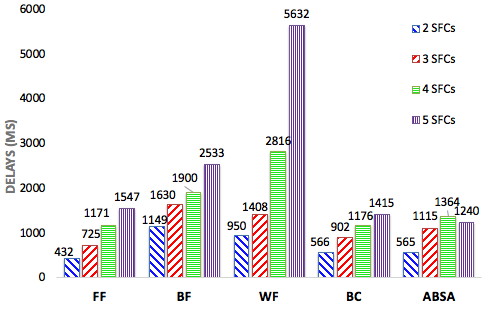
\includegraphics[width=.8\linewidth]{DelayComp.png}
	\caption{All figures require a caption, describing the content}\label{fig:myfig}
\end{figure}

Tables are best set using the booktabs package. They work by using the
table and tabular environments enclosed in each other.
Like figures, tables are floating elements that are automatically placed
by the typesetting engine. They can and should be referenced in a similar
way: Table~\ref{tab:mytable}. 

\begin{table}[b]
	\centering % Use \centering to align to center
\begin{tabular}{lcr} % [l]eft, [c]enter, [r]ight
	\toprule
	First column header & Centered text & Right aligned \\
	\midrule
	Left aligned	& Centered &	7.0 \\
	A second row	& Some text &	38.5 \\
	\bottomrule
\end{tabular}
\caption{A floating table}%
\label{tab:mytable}
\end{table}

The bibliography is managed with BibTeX. Add entries to the \verb'review-bibliography.bib'
file in the main directory. You can reference them with the cite command~\cite{Guedes03:OCT}.
BibTeX info for scientific publications is found in the common literature repositories
(Springer, Elsevier, IEEE). 

More information on LateX can be found online. There is a wikibook on LaTeX
to be found here: \url{https://en.wikibooks.org/wiki/LaTeX}. Also, the
TeX section of stackexchange.com provides answers to almost any question:
\url{https://tex.stackexchange.com/}~\cite{stackexchange}.

\newpage

\bibliography{./ml_project_bibliography} 
\bibliographystyle{apalike}

\end{document}
